\chapter{Image super-resolution}

\section{Another ill-posed problem}
\begin{itemize}
\item Image super-resolution is basically a hallucination exercise of
  a \gls{ANN}.
\item There are infinite forms of imagining
  \href{https://en.wikipedia.org/wiki/Super-resolution_imaging}{what
    could be in an image when we zoom-in a region of it}.
\end{itemize}

\section{Objective}
\begin{itemize}
\item Super-resolution is an image processing technique that
  increases the perceived quality by means of ``fabricating''
  (possibly \popup{unreal}{Invented.}) new visual information.
\item Even knowing this fact, it can help in medical imaging
  diagnosis.
\end{itemize}

\section{Nearest-neighbor interpolation \cite{gonzalez2009digital}}
\begin{itemize}
\item For a discrete image $f: \mathbb{Z}^2 \to \mathbb{R}$, the interpolation at a point 
$(x,y) \in \mathbb{R}^2$ is given by
\begin{equation}
\hat{f}(x,y) = f\!\left( \operatorname{round}(x), \operatorname{round}(y) \right),
\end{equation}
where $\operatorname{round}(x)$ returns the nearest integer value of $x$.
\end{itemize}

\begin{figure}[H]
  \vspace{-2ex}
  \centering
  \href{https://www.mrecacademics.com/DepartmentStudyMaterials/20201220-Digital%20Image%20Processing%20Notes.pdf}{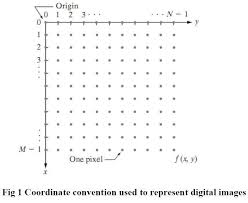
\includegraphics[width=5cm]{discrete_image}}
  \caption{Coordinates in digital images.}
  \label{fig:digital_image}
\end{figure}

\begin{figure}[H]
  \vspace{0ex}
  \centering
  \href{https://github.com/vicente-gonzalez-ruiz/medical_imaging/blob/main/notebooks/nearest_integer_interpolation.ipynb}{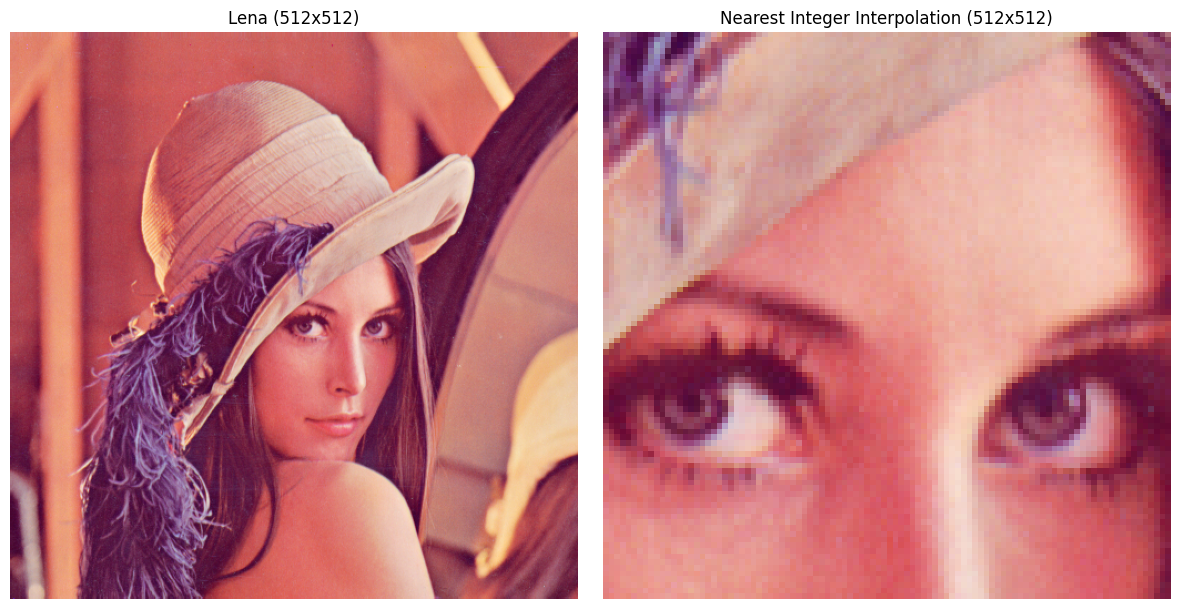
\includegraphics[width=12cm]{lena_nearest_integer}}
  \caption{Blocking generated by nearest integer interpolation.}
  \label{fig:pixel_blocking}
\end{figure}

\section{Bilinear interpolation \cite{gonzalez2009digital}}

\begin{itemize}
\item For an image $f: \mathbb{Z}^2 \to \mathbb{R}$, the bilinear interpolation at 
$(x,y) \in \mathbb{R}^2$ is
\begin{equation}
\hat{f}(x,y) = (1-\alpha)(1-\beta)\, f(i,j) 
+ \alpha(1-\beta)\, f(i+1,j) 
+ (1-\alpha)\beta\, f(i,j+1) 
+ \alpha\beta\, f(i+1,j+1),
\end{equation}
where
\[
i = \lfloor x \rfloor, \quad j = \lfloor y \rfloor, \quad
\alpha = x - \lfloor x \rfloor, \quad \beta = y - \lfloor y \rfloor.
\]

\newpage
\item Smooth transitions, commonly used in \gls{CT}/\gls{MRI} resampling.
\end{itemize}

\begin{figure}[H]
  \vspace{-1ex}
  \centering
  \href{https://github.com/vicente-gonzalez-ruiz/medical_imaging/blob/main/notebooks/bilinear_interpolation.ipynb}{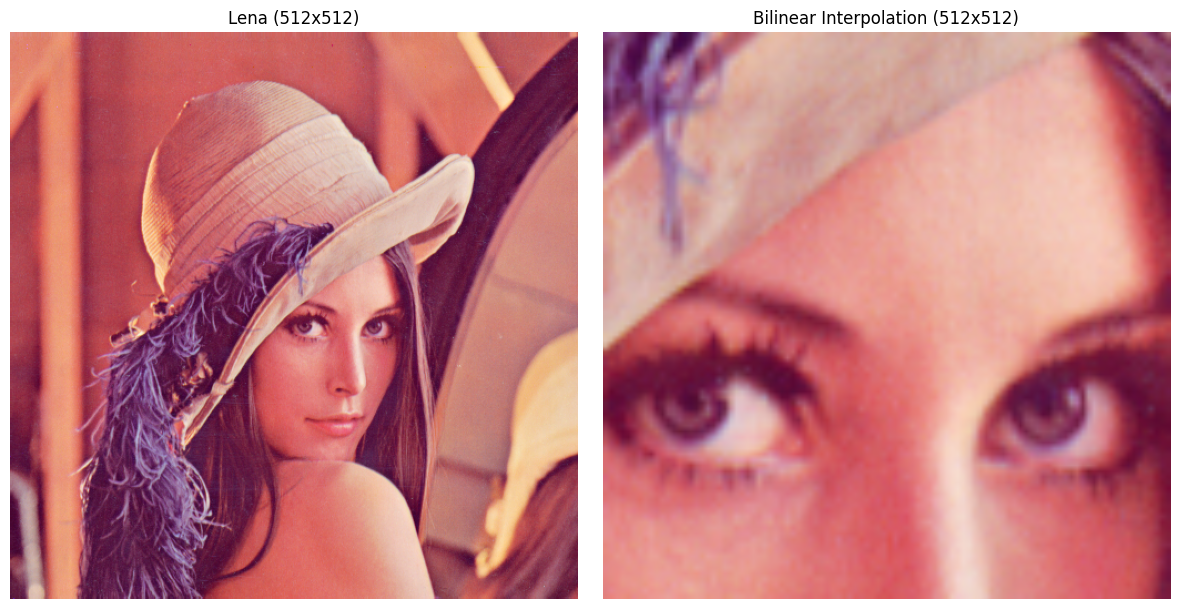
\includegraphics[width=11cm]{lena_bilinear}}
  \caption{Bilinear interpolation example.}
  \label{fig:bilinear_interpolation}
\end{figure}

\section{\gls{ESRGAN} \cite{wang2018esrgan}}
\begin{itemize}
\item ESRGAN is a \popup{deep}{349 convolutional layers.} \gls{CNN}
  $G_\theta$ trained with adversarial and perceptual losses to
  \popup{hallucinate}{Imagine.} realistic high-frequency image
  details.
\end{itemize}

\begin{figure}[H]
  \vspace{0ex}
  \centering
  \href{https://arxiv.org/abs/2207.08036}{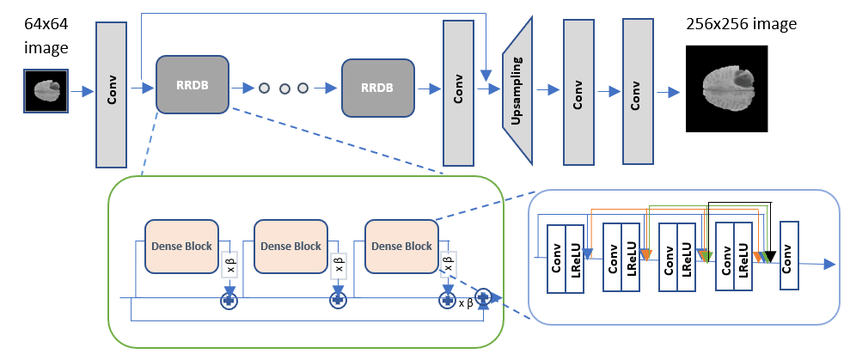
\includegraphics[width=11cm]{Generator-Architecture-of-Real-ESRGAN}}
  \caption{$G_\theta$, the generator used in \gls{ESRGAN}.}
  \label{fig:ESRGAN_generator}
\end{figure}

\begin{itemize}
\item $G_\theta$ performs
  \begin{equation}
    \hat{I}_{\text{HR}} = G_\theta(I_{\text{LR}}),
  \end{equation}
  where $I_{\text{LR}}$ is the low-resolution input image and
  $\hat{I}_{\text{HR}}$ is the \popup{high-resolution}{4x in the
    figure.} output image.
\end{itemize}

\section*{Adversarial training}

\begin{figure}[H]
  \vspace{0ex}
  \centering
  \href{https://semiengineering.com/knowledge_centers/artificial-intelligence/neural-networks/generative-adversarial-network-gan/}{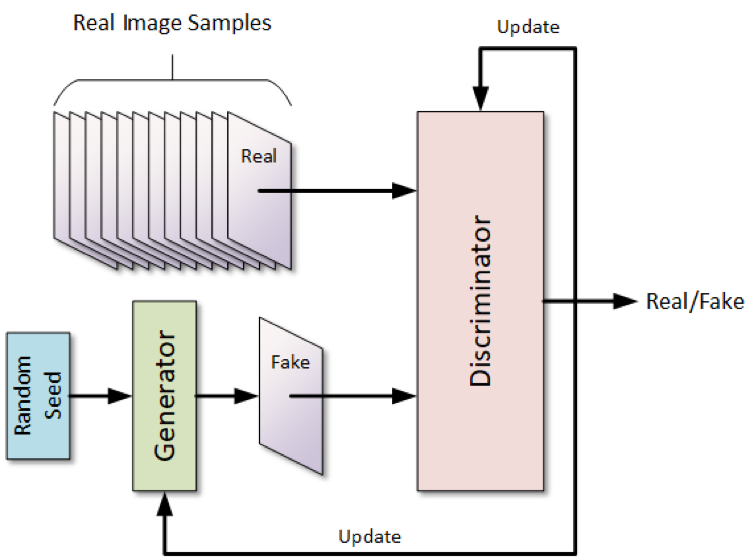
\includegraphics[width=8cm]{GAN}}
  \caption{The \gls{ESRGAN} network.}
  \label{fig:ESRGAN}
\end{figure}

\begin{itemize}
\item \popup{Unsupervised learning}{This is true for all GANs.} that
  utilize two neural networks:
  \begin{enumerate}
  \item \textbf{Generator} ($G_\theta$): Using random data or a seed image,
    generate \popup{fake}{Unreal.} images.
  \item \textbf{Discriminator} ($D_\phi$): Try to determine if the generated
    image is real or not.
  \end{enumerate}
\item In each iteration, and independently of who wins, both, the
  discriminator and the generator are retrained (updated) considering
  the result.
\item The training ends when generator has \popup{no
    idea}{There is a 50-50 chance of success.}  about the veracity of the image
  he receives.
\item \glspl{GAN} can be trained for generate any kind of content,
  such as for example,
  \href{https://thispersondoesnotexist.com/}{faces}).
\end{itemize}

\section*{Training of the discriminator}
\begin{itemize}
\item The discriminator’s objective function
\begin{equation}
  \mathcal{L}_D(\phi) = 
  \mathbb{E}\big[ \log D_\phi(I_{\text{HR}}) \big] 
  + \mathbb{E}\big[ \log (1 - D_\phi(G_\theta(I_{\text{LR}}))) \big],
\end{equation}
is maximized when it outputs a probability close to 1 for real HR
images and close to 0 for fake HR images. We have that:
\begin{enumerate}
\item $\phi$ represents the \popup{parameters}{Weights of the ANN.} of
  the discriminator.
\item $\mathbb{E}[x]$ is the
  \popup{expectation}{Basically the mean.} of the sequence of values
  $x$ where $x_i$ is a HR image.
\item $G_\theta(I_{\text{LR}})$ is the fake image.
\item $ D_\phi(G_\theta(I_{\text{LR}}))$ is the discriminator decision for the fake image.
\item $\log(1 - D_\phi(G_\theta(I_{\text{LR}})))$ is very negative if
  the decision is one (the generated image is fake, and I guess that
  is real), and is zero if the decision is 0 (the generated image is
  fake, and I guess that is fake). Therefore, each time the
  discriminator fails, the objective is \popup{reduced}{Remember that
    we want to maximize this function.}.
\item $\log D_\phi(I_{\text{HR}})$ is \popup{zero}{Good :-)} if the
  discriminator's guess is correct (I recognized that $I_{\text{HR}}$
  is a real image), and very \popup{negative}{Bad :-(} if the guess is
  incorrect.
\end{enumerate}
\end{itemize}

\section*{Training of the generator}
\begin{itemize}
\item The generator try to minimize
\begin{equation}
\mathcal{L}_G(\theta) = 
\lambda_{\text{adv}} \, \mathcal{L}_{\text{adv}}(\theta) \;+\;
\lambda_{\text{con}} \, \mathcal{L}_{\text{con}}(\theta) \;+\;
\lambda_{\text{pix}} \, \mathcal{L}_{\text{pix}}(\theta),
\end{equation}
where
\begin{equation}
  \mathcal{L}_{\text{adv}}(\theta) = - \mathbb{E}\big[ \log D_\phi(G_\theta(I_{\text{LR}})) \big]
\end{equation}
is the adversarial loss,
\begin{equation}
\mathcal{L}_{\text{con}}(\theta) = \mathbb{E}\left[ \big\| \Phi(G_\theta(I_{\text{LR}})) - \Phi(I_{\text{HR}}) \big\|_2^2 \right]
\end{equation}
is the content (perceptual) loss, and
\begin{equation}
\mathcal{L}_{\text{pix}}(\theta) = \mathbb{E}\left[ \| G_\theta(I_{\text{LR}}) - I_{\text{HR}} \|_1 \right]
\end{equation}
is the pixel loss, where $\lambda_{\text{adv}}, \lambda_{\text{con}},$
and $\lambda_{\text{pix}}$ are three hyperparameters that control the
weight of each loss, $\theta$ represents the parameter of the
generator, $\Phi(\cdot)$ a feature extraction function (usually the
output of an intermediate layer), $\big\|\cdot\big\|_2^2$ the squared
Euclidean norm (close to the \gls{MSE}). and $\|\cdot\|_1$ is the \popup{L1 norm}{called the
  Manhattan norm or taxicab norm}.

\end{itemize}

\begin{figure}[H]
  \vspace{0ex}
  \centering
  \href{https://github.com/vicente-gonzalez-ruiz/medical_imaging/blob/main/notebooks/ESRGAN.ipynb}{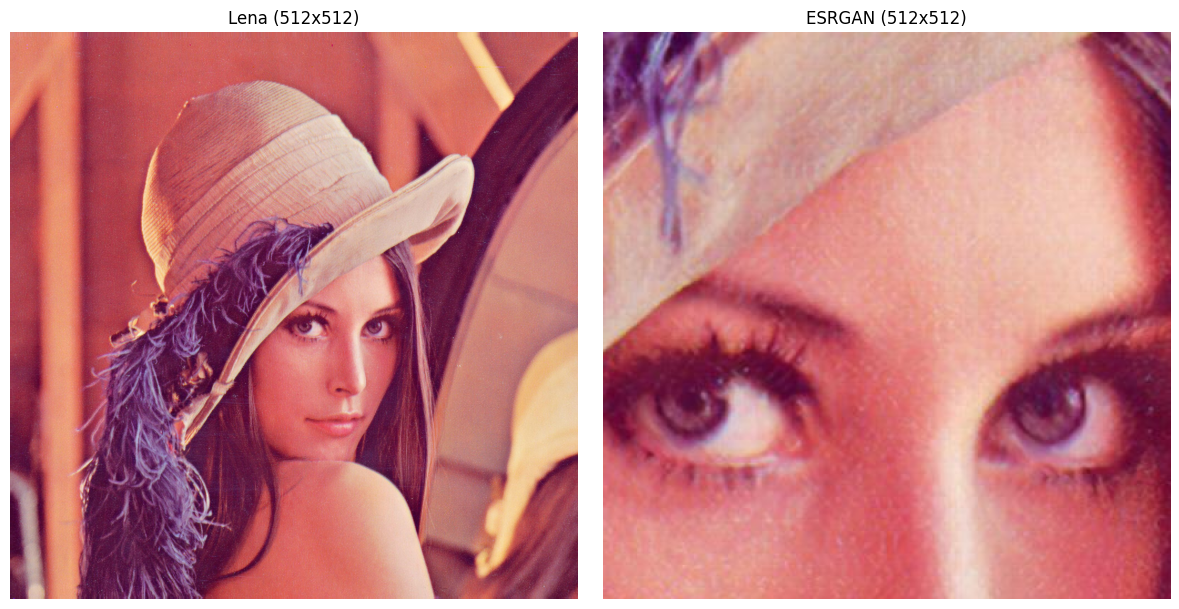
\includegraphics[width=12cm]{lena_ESRGAN}}
  \caption{A super-resolution example with \gls{ESRGAN}.}
  \label{fig:ESRGAN_example}
\end{figure}

